\subsubsection{Transaction Execution}
\label{sec:tx-execution}

The transaction execution is the mechanism through which the world state is
updated. It represents a transition from one valid state to another valid state.

A transaction specifies a \emph{receiver} and the \emph{value} that must be
transferred from the sender to the receiver. Moreover, to avoid the abuse of the
resources (CPU and storage) of the full nodes forming the network and to ensure
that all executions terminate, the concept of \emph{gas} is introduced. In
this execution model each action that must be performed by the members of the
network has an associated cost expressed in gas. In particular, each EVM
byte-code instruction, increase in the storage space by a contract and the
transaction itself have a fixed associated cost. A transaction specifies its
\emph{gas price} and its \emph{gas limit}. The former is the price of a unit
of gas and is bound to a particular execution. The higher this price the higher
the possibility that the miner will include this transaction in the blockchain.
Usually the miners advertise the minimum gas price they are willing to accept.
The latter is the maximum amount of gas the executor is ready to consume for
this particular execution.

\begin{figure}[h!]
	\begin{center}
		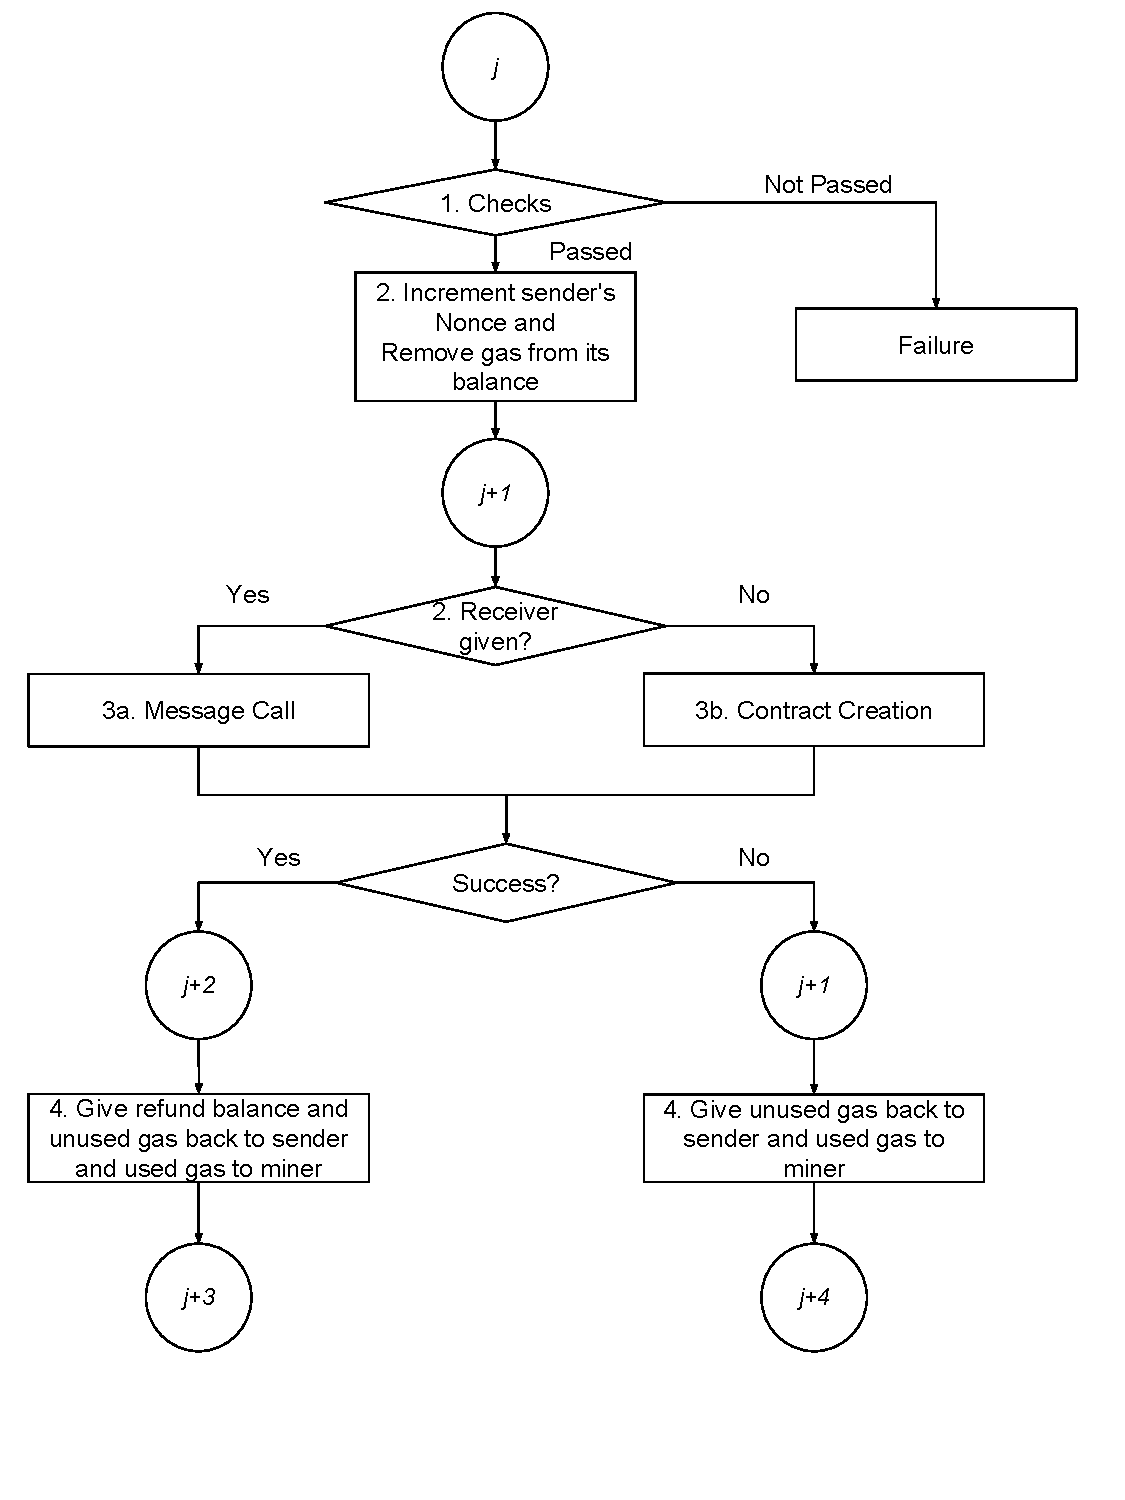
\includegraphics[width=0.60\textwidth]{./res/img/transaction-execution.pdf}
	\end{center}
	\caption{The steps of the transaction execution algorithm.}
	\label{fig:tx:execution}
\end{figure}

\autoref{fig:tx:execution} summarizes the steps of the algorithm for the
transaction execution:
\begin{enumerate}
	\item The transaction has to pass some simple validity checks, e.g.\ the
	transaction should be a well-formed RLP encoded string and the initiator of
	the transaction should have a balance big enough to afford the transaction.
	Moreover, since a transaction should be included in a block and the block
    has in turn its own gas limit, it should be also true that the sum of the
	accumulated gas used by the already included transactions and the gas limit
    of this transaction are smaller than the block's gas limit. If these checks
    fail, the transaction is simply not included in the block in case of miner
    or it indicates that the block is invalid in case of verifier.
	\item The nonce of the initiator of the transaction is incremented by one
    and its balance is reduced by the product of the gas limit and the gas
    price. This modification to the state is irreversible.
	\item Now, depending on whether the receiver address is given or not we should
	make a distinction between:
	\begin{enumerate}[label=\alph*.]
		\item Message Calls (\autoref{sec:message-call}) and;
		\item Contract Creation (\autoref{sec:contract-creation}).
	\end{enumerate}
	During the execution of the message call or contract creation the system keeps
	track of the \emph{transaction substate}, i.e., some important information
	that are later used to complete the state transition. The transaction
    substate includes the \emph{touched accounts}, the set of accounts that
    will be discarded following the completion (\emph{self-destruct set}) and
    the \emph{refund balance}, that is an amount of gas that is incremented by
	removing elements from the world state, e.g., by setting a non-zero value
    to a zero value in the storage or by removing a contract from the state.
	\item Once the message call or the contract creation are concluded, the sum
    of the remaining gas and the refund balance are refunded to the initiator
    of the transaction at the transaction's gas price\footnote{This sum cannot
    exceed the initial allocated price~\cite{wood2018ethereum}, in other words
    the refund balance can be used to mitigate the transaction cost, but not to
    profit.}. If the message call or contract creation did not complete
    successfully, the state is reverted and the refund balance is zeroed, since
    its modifications to the state are not considered. The gas used is given to
    the beneficiary address (i.e., the miner) who built and finalized the
    block. Finally, the self-destruct set and the touched accounts that became
    empty or dead after the transaction should be deleted from the world state.
\end{enumerate}


